\onehalfspacing

%%CAPITOLO 3: =======================================

\chapter{Implementazione e sperimentazione}

\section{Architettura del sistema}\label{sec:arch}
Il sistema � stato scritto interamente con il linguaggio di programmazione \textit{Java} in ambiente \textit{Eclipse}.

La word cloud viene generata a partire da un file di testo (formato \textit{.txt}) in input. Tuttavia, il software � dotato di una classe, SrtFileCleaner, che permette di ricevere in input un file di testo in formato \textit{.srt}, che � la rappresentazione di un generico sottotitolo, con relativi timestamp, e lo ripulisce, in modo da ottenere un semplice file di testo. Il supporto a questo tipo di file � utile perch� la word cloud dinamica si pu� creare a partire da video che contengono il relativo sottotitolo (ad esempio, a partire dai video di YouTube).

La fase di pre-processing inizia con l'elaborazione del testo. A tal fine, � stato utilizzato il toolkit open source \textit{Apache OpenNLP}\cite{opennlp}, basato su tecniche di Machine Learning per l'elaborazione del linguaggio naturale. Questo toolkit consente l'esecuzione delle varie fasi che preparano il testo in input all'algoritmo di estrazione delle keywords: rilevamento delle frasi, suddivisione del testo in token, stemming e rimozione delle stop word. Per ogni fase si utilizzano dei modelli (forniti dalla libreria) per l'elaborazione della lingua inglese, ma anche altre lingue sono supportate. 

L'elaborazione del testo, con conseguente estrazione delle keywords, � gestita dalla classe \textit{Document}, il cui costruttore ha come parametri il testo da elaborare, l'algoritmo di rilevamento delle frasi, il tokenizer, l'algoritmo di stemming e la lista delle stop word (figura \ref{class:doc}). Nella nostra implementazione l'algoritmo di stemming utilizzato � il Porter Stemmer, fornito dalla libreria. Il metodo che elabora il testo � \textit{parse()}, il quale predispone in modo opportuno la lista delle parole da cui l'algoritmo di ranking estrarr� le parole pi� rilevanti. 
\begin{figure}
\centering
{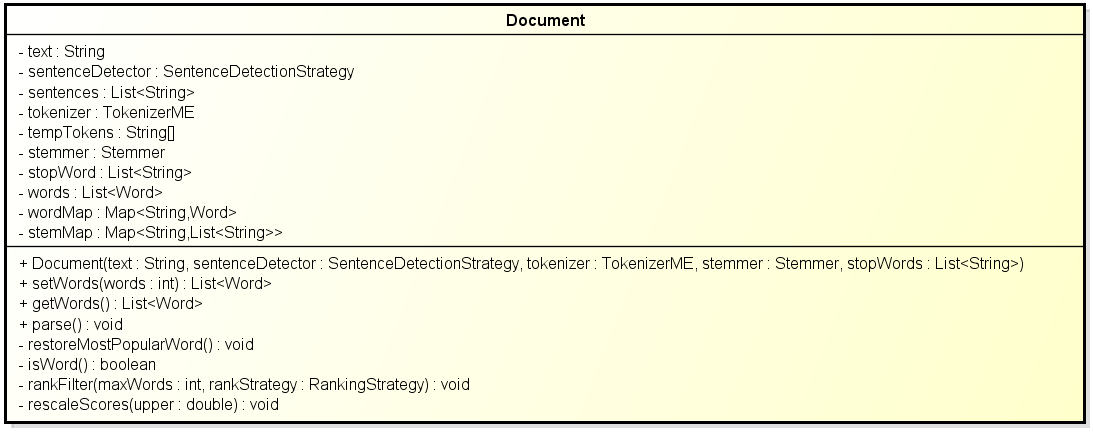
\includegraphics[scale=0.6]{img/impl_test/class_doc.png}}
\caption[Class diagram delle classe Document.]{Class diagram delle classe Document.}
\label{class:doc}
\end{figure}
Il ranking e la conseguente estrazione delle parole � gestita dal metodo \textit{rankFilter(int maxWords,RankingStrategy rankStrategy)}, i cui parametri sono il numero di parole da estrarre e l'algoritmo di ranking, attraverso cui viene chiamato il metodo \textit{rank(Document document)}, che esegue la classificazione delle parole. Tale metodo � dichiarato nell'interfaccia \textit{RankingStrategy} ed � realizzato dalle classi che estendono \textit{RankingStrategy}, le quali rappresentano i diversi algoritmi di estrazione delle keywords descritti nel precedente capitolo (figura \ref{strategy:rank}). L'utilizzo del pattern \textbf{Strategy}\cite{gof}, rende l'architettura parametrica rispetto agli algoritmi di estrazione delle parole (lo stesso avviene con gli algoritmi impiegati nelle fasi successive del processo di creazione della word cloud).
\begin{figure}
\centering
{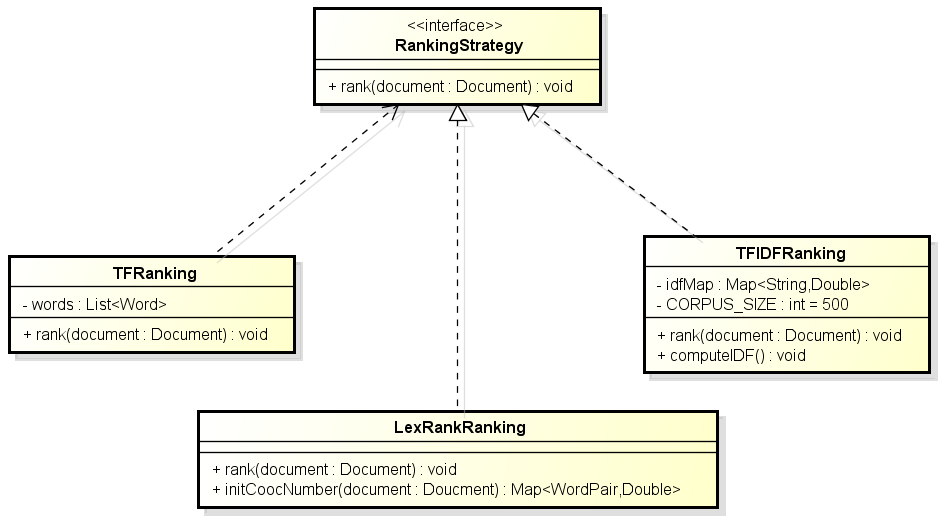
\includegraphics[scale=0.7]{img/impl_test/rank_strategy.png}}
\caption[Classi coinvolte nell'estrazione delle parole.]{Classi coinvolte nell'estrazione delle parole. Nell'implementazione dell'algoritmo TF-IDF, � stato usato il corpus Brown\cite{wiki:browncorpus}.}
\label{strategy:rank}
\end{figure}

Ogni parola � un'istanza della classe \textit{Word}, che gestisce diverse caratteristiche di una parola, tra cui la radice, il punteggio e le sue variazioni, la lista di frasi in cui essa compare ecc... (figura \ref{class:word}). 
\begin{figure}
\centering
{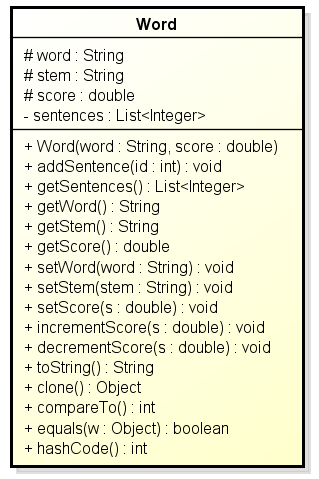
\includegraphics[scale=1]{img/impl_test/class_word.png}}
\caption[Class diagram delle classe Word.]{Class diagram delle classe Word.}
\label{class:word}
\end{figure}

Una volta ottenute le parole estratte, si procede al calcolo della similarit�, tramite uno degli algoritmi di similarit� definiti in precedenza. Si utilizza un approccio parametrico come per gli algoritmi di ranking (figura \ref{strategy:simil}).
\begin{figure}
\centering
{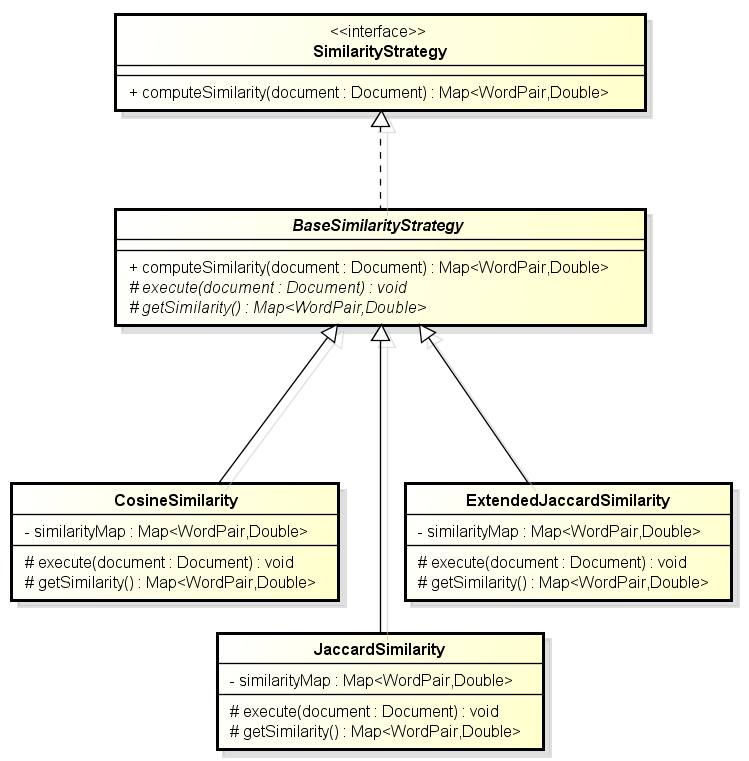
\includegraphics[scale=0.6]{img/impl_test/simil_strategy.png}}
\caption[Classi coinvolte nel calcolo della similarit� tra parole.]{Classi coinvolte nel calcolo della similarit� tra parole.}
\label{strategy:simil}
\end{figure}

Ottenute la lista delle parole pi� rilevanti e la similarit� a coppie, si procede con la costruzione del grafo tramite la classe \textit{WordGraph}, il cui costruttore ha come parametri la lista delle parole e la mappa delle similarit� tra coppie di parole. Il generico oggetto \textit{WordGraph} � il parametro degli algoritmi di layout. 
\section{Risultati sperimentali}\label{sec:test}